\chapter{Хэрэгжүүлэлт}

Энэхүү бүлэгт өмнө нь гарсан интерфэйс дизайн, системийн архитектур болон диаграмуудыг хэрэгжүүлж хэрхэн бүтээгдэхүүн болгон гаргасан талаараа бичлээ. Хэрэгжүүлэлт хийх үе шатаа ерөнхийд нь

\begin{itemize}
	\item Хөгжүүлэлтийн орчноо бэлдэх
	\item Front-end болон Back-end хөгжүүлэлт
	\item Серверт байршуулах /Deploy/
\end{itemize}

гэсэн алхмуудад хувааж гүйцэтгэсэн ба доор ажлуудаасаа гол гэсэн зүйлсээ нэгтгэн орууллаа.

\section{Хөгжүүлэлтийн орчныг бэлдэх}
\label{section:backend}

Ашиглах технологийн хувьд Next.js, Prisma ORM, PostgreSQL ашиглах учир хамгийн эхлээд өгөгдлийн сангаа Local хост дээрээ бэлдэж, дараа нь Next.js фрэймворкоо суулган шаардлагатай тохиргоонуудыг хийлээ. Үүний дараагаас Prisma ORM-ээ суулгаж, урьдчилж бэлдсэн Next.js төсөл дээрээ орууллаа. 

Мөн кодын хувилбараа хадгалж, хөгжүүлэлтийн үе шатаа цэгцтэй авч явахын тулд  Version Control дээрээ Git, Github.com-г ашиглан хувийн repository үүсгэлээ. 

\clearpage
\begin{figure}[h]
	\centering
	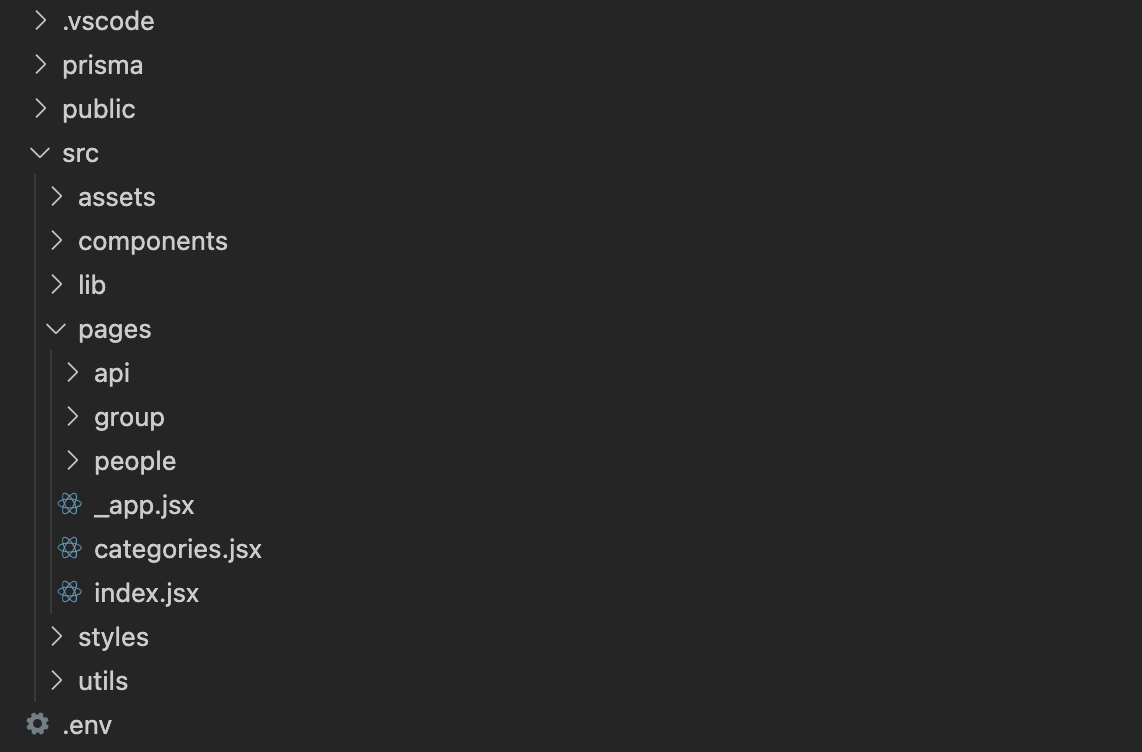
\includegraphics[width=10cm]{images/implement/file-structure.png}
	\caption{Төслийн файлын бүтэц}
	\label{fig:file-structure}
\end{figure}

Next.js дээр файлын бүтцээ дараах байдлаар бэлдэв. Back-end болон Front-end-ээ уг технологийг ашиглан хийж буй учир уг бүтэц дотор back-end хэсгийн код багтсан байгаа.

\begin{itemize}
	\item \textbf{prisma} хавтаст цаашдаа ашиглах schema байршина
	\item \textbf{public} хавтаст төслийн хүрээнд ашиглах статик файлууд /зураг, icon/ байна
	\item \textbf{src} хавтаст төслийн бүх компонент, хуудсаад болон back-end код давхар хадгалагдана
\end{itemize}

\section{Код хөгжүүлэлт}

Хэрэгжүүлэлтийн хувьд маш олон интерфэйс, код орсон тул доор хэсэгт нүүр хуудасны бусад хүмүүсийн оруулсан нийтлэлийг харуулдаг хэсгийг тайлбарлав.

\subsection{Гаргасан интерфэйсийнхээ дагуу хэрэглэгчид харагдах хэсгийг өрсөн нь}

Front-end хөгжүүлэлт дээр урьдчилж интерфэйс дизайныг гаргасан нь вебийн бүх компонент, тэдгээр хаана байрших гээд олон зүйлийг тодорхой болгож өгсөн нь давуу тал болж өгсөн. Иймд хамгийн эхлээд бэлдсэн хөгжүүлэлтийн орчин дээрээ үндсэн хуудсууд болон дотор нь ашиглаж буй компонентуудыг статик байдлаар өрөв. 

\begin{lstlisting}[language=Javascript, caption=Хэрэглэгчийн оруулсан холбоосын харагдах компонент, frame=single]
	export const Card = ({
  href,
  type,
  site_url,
  og_title,
  og_image,
  author_name,
  author_profile,
  vote_count,
  tags,
}) => {
  return (
    <Link href={href} target="_blank">
      <div className="cursor-pointer space-y-2 rounded-lg border border-gray200 bg-gray300 p-3.5 transition-all duration-300 hover:border-gray100 hover:bg-white hover:shadow-sm">
        <div className="flex items-center gap-1 text-sm font-normal text-description">
          <LinkIcon />
          {site_url}
        </div>
	       
					...

          <div className="order-last flex items-center gap-1 text-sm text-description">
            <VoteBtn type="up" />
            <VoteBtn type="down" />
          </div>
        </div>
      </div>
    </Link>
  );
};
			
\end{lstlisting}


\subsection{Prisma ORM ашиглаж өгөгдлийн сантайгаа харьцах нь}

Хамгийн түрүүнд өгөгдлийн сангийн схемийнхээ дагуу \textbf{prisma/schema.prisma} файл дээр өгөгдлийн сан дээр үүсгэх хүснэгт, багануудын бүх нөхцлийг бичиж хэрэглэгчийн оруулсан нийтлэлийн өгөгдлийг хадгалах \textbf{Post} гэсэн хүснэгтийг үүсгэнэ.

\begin{lstlisting}[language=Javascript, caption=Өгөгдлийн сангийн хүснэгтийг Prisma ашиглан үүсгэх, frame=single]
	generator client {
		provider = "prisma-client-js"
	}
	
	datasource db {
		provider = "postgresql"
		url      = env("DATABASE_URL")
	}
	
	model Post {
		id       Int    @id @default(autoincrement())
		siteUrl  String
		ogTitle  String
		ogImage  String
		authorId Int
		author   User   @relation(fields: [authorId], references: [id], onDelete: Cascade)
		groupId  Int?
		group    Group? @relation(fields: [groupId], references: [id])
		tags       Tag[]
		categories Category[]
		createdAt DateTime @default(now())
		updatedAt DateTime @updatedAt
	}	

	...

\end{lstlisting}

Уг файлыг \textbf{migration} хийсний дараа бичсэн моделийн дагуу өгөгдлийн сан дээр \textbf{Post} хүснэгт үүссэн. 

\begin{figure}[h]
	\centering
	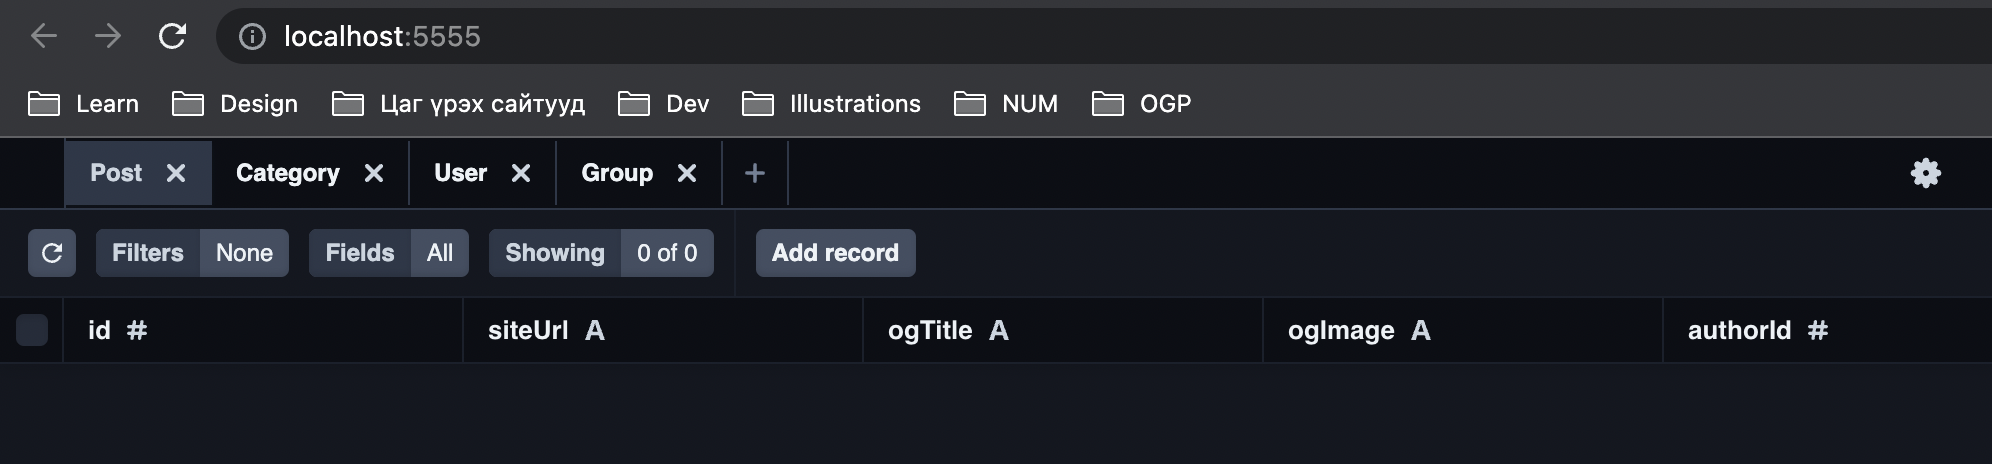
\includegraphics[width=10cm]{images/implement/table.png}
	\caption{Post хүснэгтийн харагдац}
	\label{fig:table}
\end{figure}

\subsection{Нийтлэлийн өгөгдлийг front-end хэсэг рүү илгээх end point гаргах нь}

Back-end-н түрүүн хэлсэнчлэн шууд Next.js фрэймворк дээрээ \textbf{/api/posts/index.js} гэсэн файл үүсгэж Prisma-гаа ашиглан өгөгдлийн сангаасаа өгөгдлөө авч ашиглана.

\begin{lstlisting}[language=Javascript, caption=Next.js дээрээ end point гаргах, frame=single]
	import { NextApiRequest, NextApiResponse } from 'next'
	import prisma from '../../../lib/prisma'
	
	export default async function handle(req: NextApiRequest, res: NextApiResponse) {
		const blogsDB = await prisma.post.findMany({
			include: {
				author: true,
				tags: true
			}
		})
	
		const blogs = blogsDB
			.map(b => {
				return {
					href: "#",
					type: "single",
					site_url: b.siteUrl,
					og_title: b.ogTitle,
					og_image: b.ogImage,
					vote_count: 1301,
					author: {
						username: b.author.username,
						profile: b.author.profileImg,
						uri: "#"
					},
					tags: b.tags.map(t => t.name),
				}
			})
	
		res.json(blogs)
	}

	...

\end{lstlisting}

Уг кодны үр дүнд дараах JSON object үүссэнийг Postman ашиглаж GET хүсэлт тавин харууллаа.

\begin{figure}[h]
	\centering
	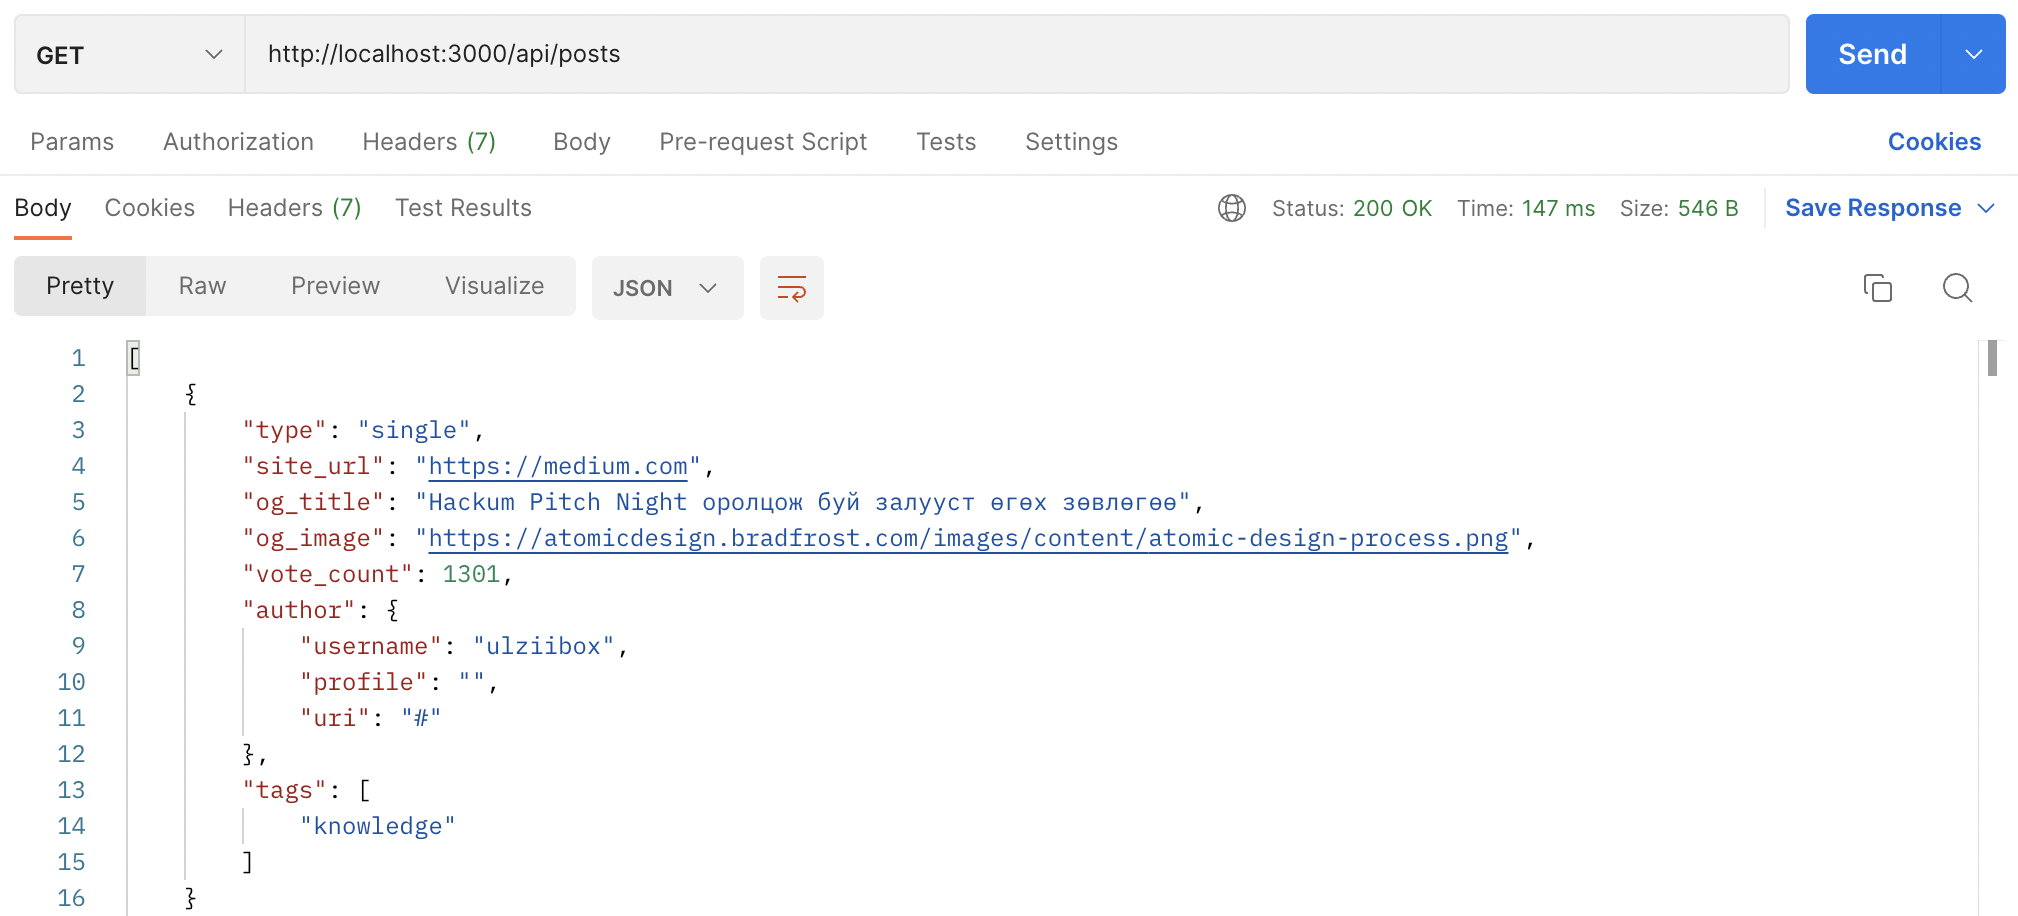
\includegraphics[width=13cm]{images/implement/endpoint.png}
	\caption{Нийтлэлийн жагсаалтыг агуулсан JSON Object}
	\label{fig:endpoint}
\end{figure}

\subsection{Front-end хэсэг дээр гаргасан End point-оо ашиглах}

Одоо Front-end хэсэг дээрээ нийтлэлийн жагсаалтуудыг авч нүүр хуудаст зурж харуулах шаардлагатай. Үүний тулд axios хүсэлтийг ашиглаж өгөгдлөө авч өмнө нь үүсгэсэн \textbf{Card} компонентдоо шаардлагатай \textbf{props}-уудыг дамжуулж, нийтлэлийг \textbf{map} функээр харуулж байгаа. 

\begin{lstlisting}[language=Javascript, caption=Card компонентод props-р утга дамжуулах, frame=single]
	
	...
	const router = useRouter();

  useEffect(() => {
    setPosts(() => {
      return formatPosts(DEMO_POSTS);
    });
    setCategories([
      {
        id: 0,
        name: "Бүгд",
      },
      ...CATEGORIES,
    ]);
  }, []);

	... 

	{posts.map((item) => {
		if (item.type === "single") {
			return (
				<Card
					key={item.post.id}
					site_url={item.post.site_url}
					og_title={item.post.og_title}
					og_image={item.post.og_image}
					author_name={item.post.author.username}
					author_profile={item.post.author.profile_img}
					vote_count={item.post.vote_count}
					tags={item.post.tags}
					href={item.post.href}
				/>
			);
		}
	}}

	...

\end{lstlisting}

\subsection{Үр дүн}

Дээрх үйлдлүүд нь манай төслийг хэрхэн ажиллаж буйг тоймлон харуулсан ба бусад хүмүүсийн оруулсан нийтлэл хэрэглэгчийн хэсгийн нүүр хуудас дээр дараах байдалтай харагдана. 

\begin{figure}[h]
	\centering
	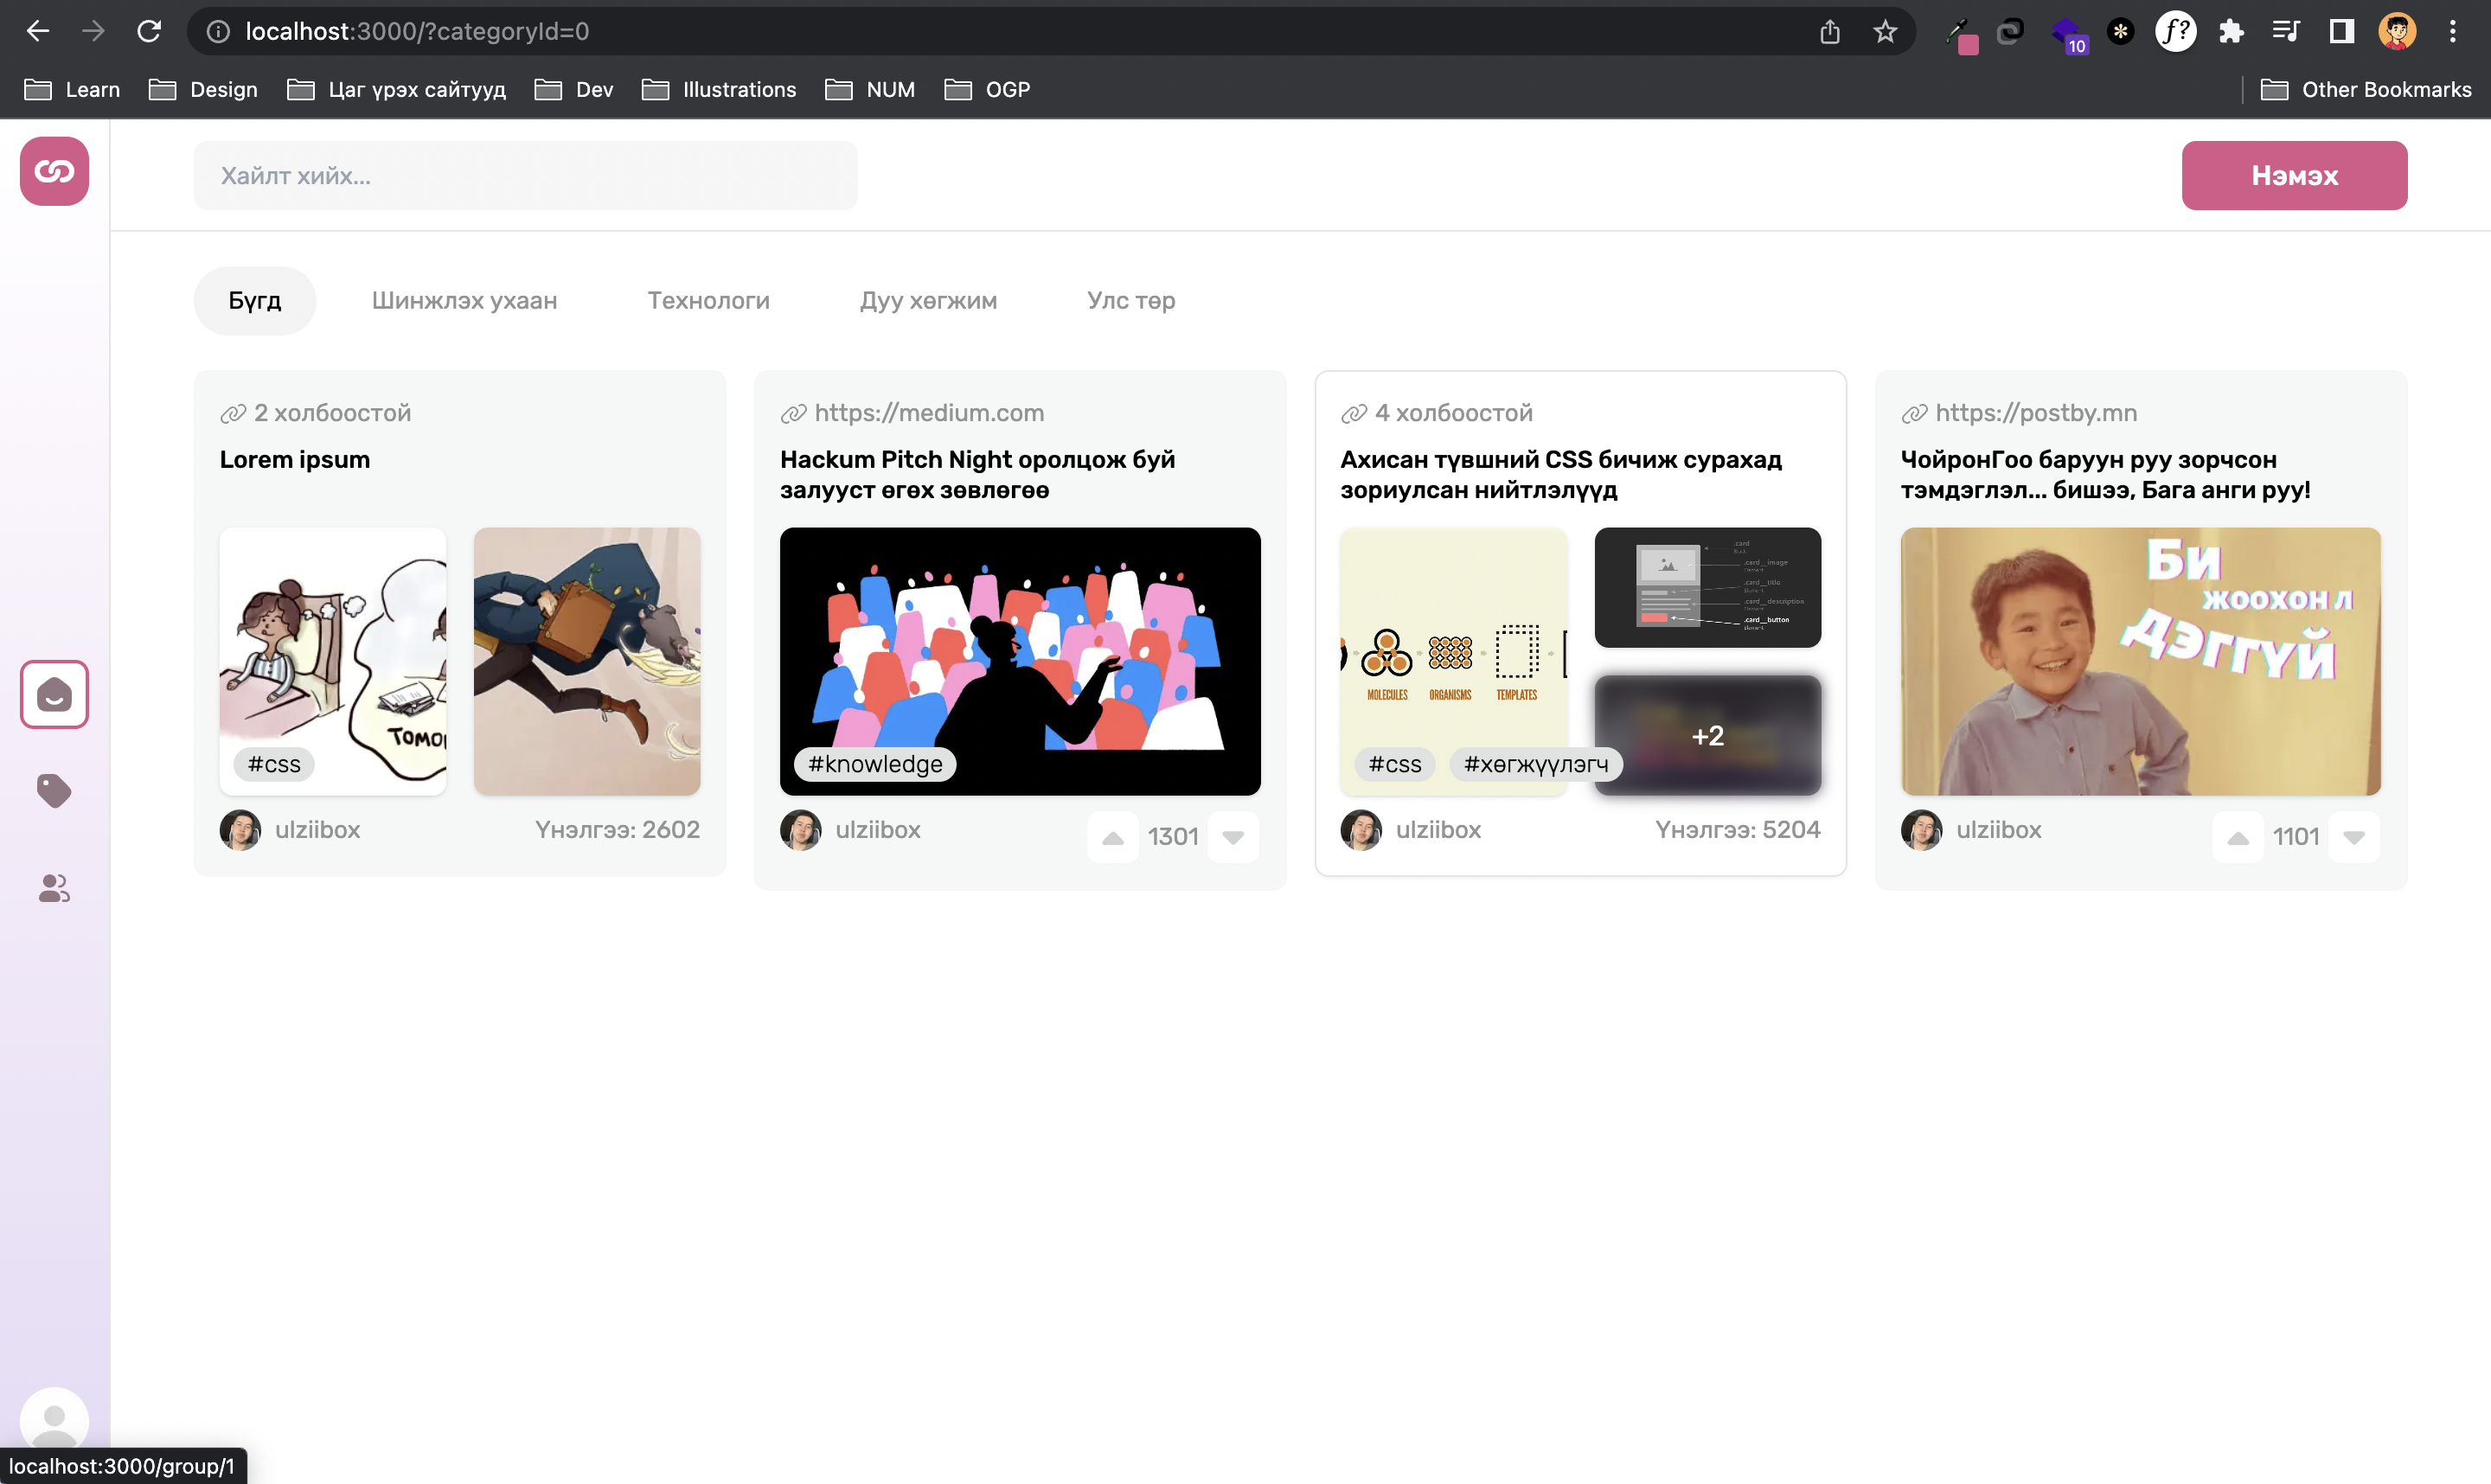
\includegraphics[width=13cm]{images/implement/home-page.png}
	\caption{Нүүр хуудас}
	\label{fig:home-page}
\end{figure}

Мөн цаашид дээрх байдлаар бусад хэсгүүдийг хийж гүйцэтгэх байгаа ба жишээ болгон бусад зурагдсан хуудсуудаас харуулъя.

\begin{figure}[h]
	\centering
	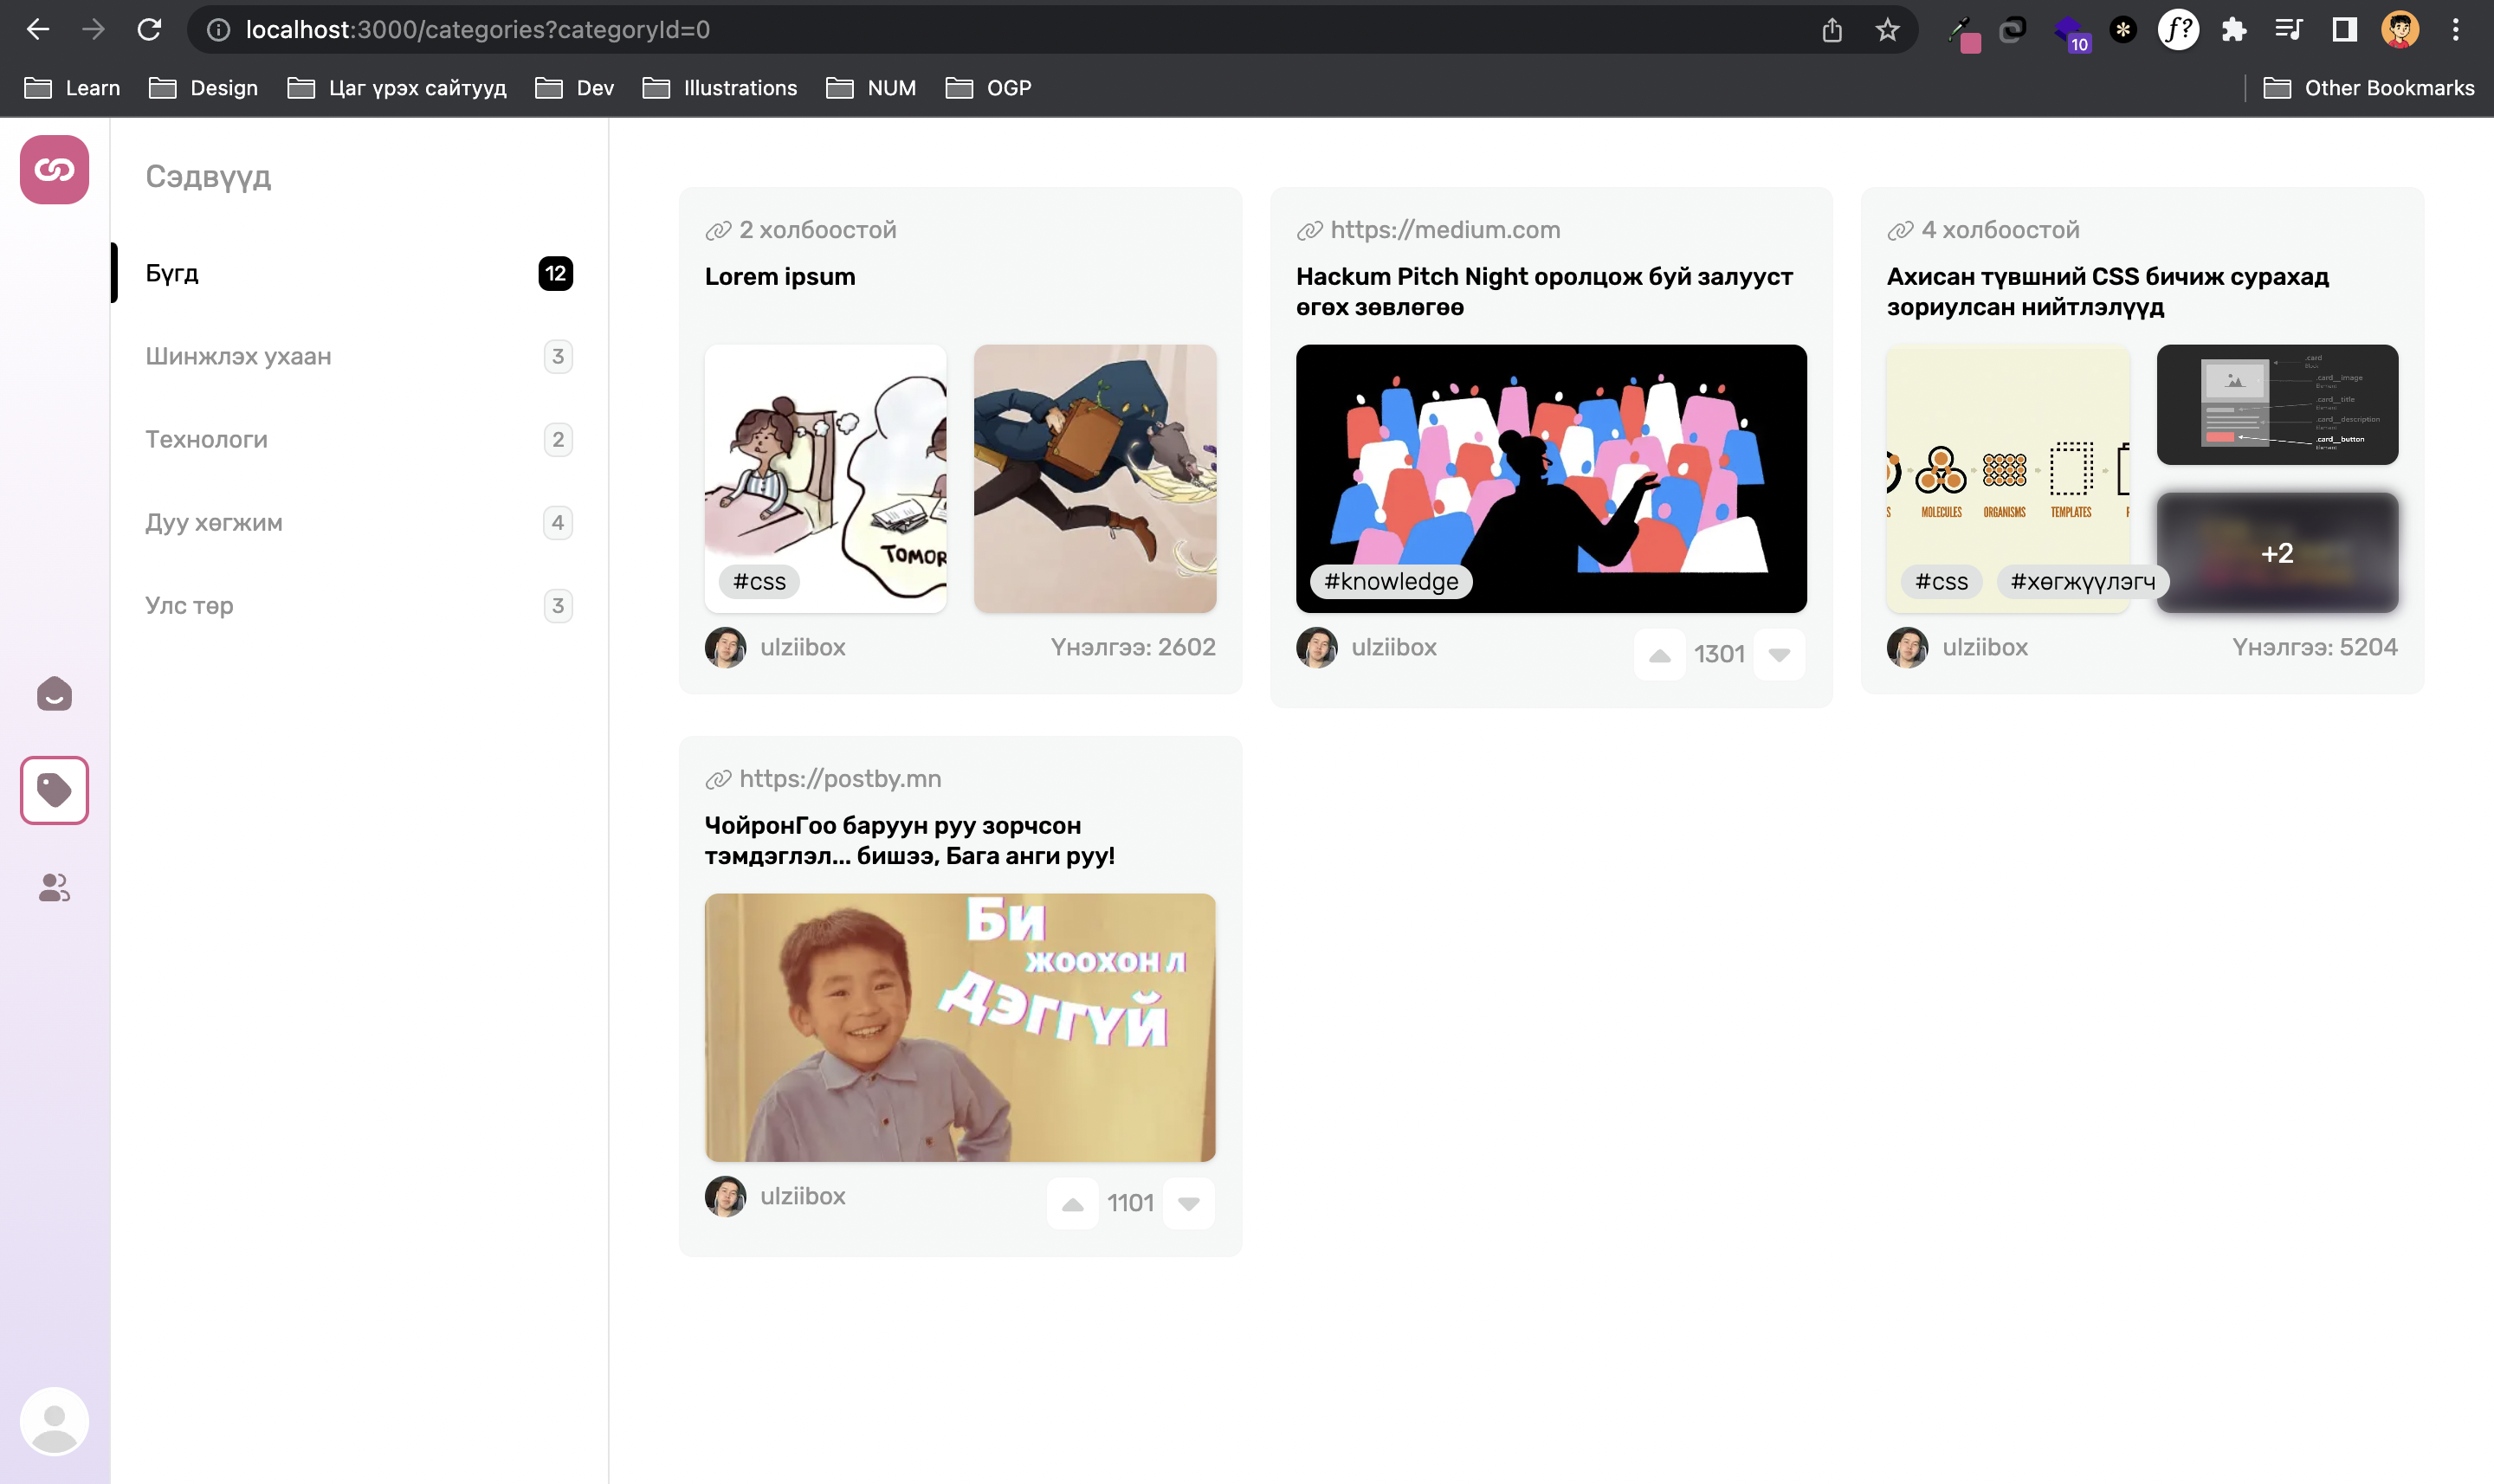
\includegraphics[width=13cm]{images/implement/category.png}
	\caption{Платформ дээрх сэдвүүдийн жагсаалт болон бүх нийтлэлийг харах}
	\label{fig:category}
\end{figure}

\begin{figure}[h]
	\centering
	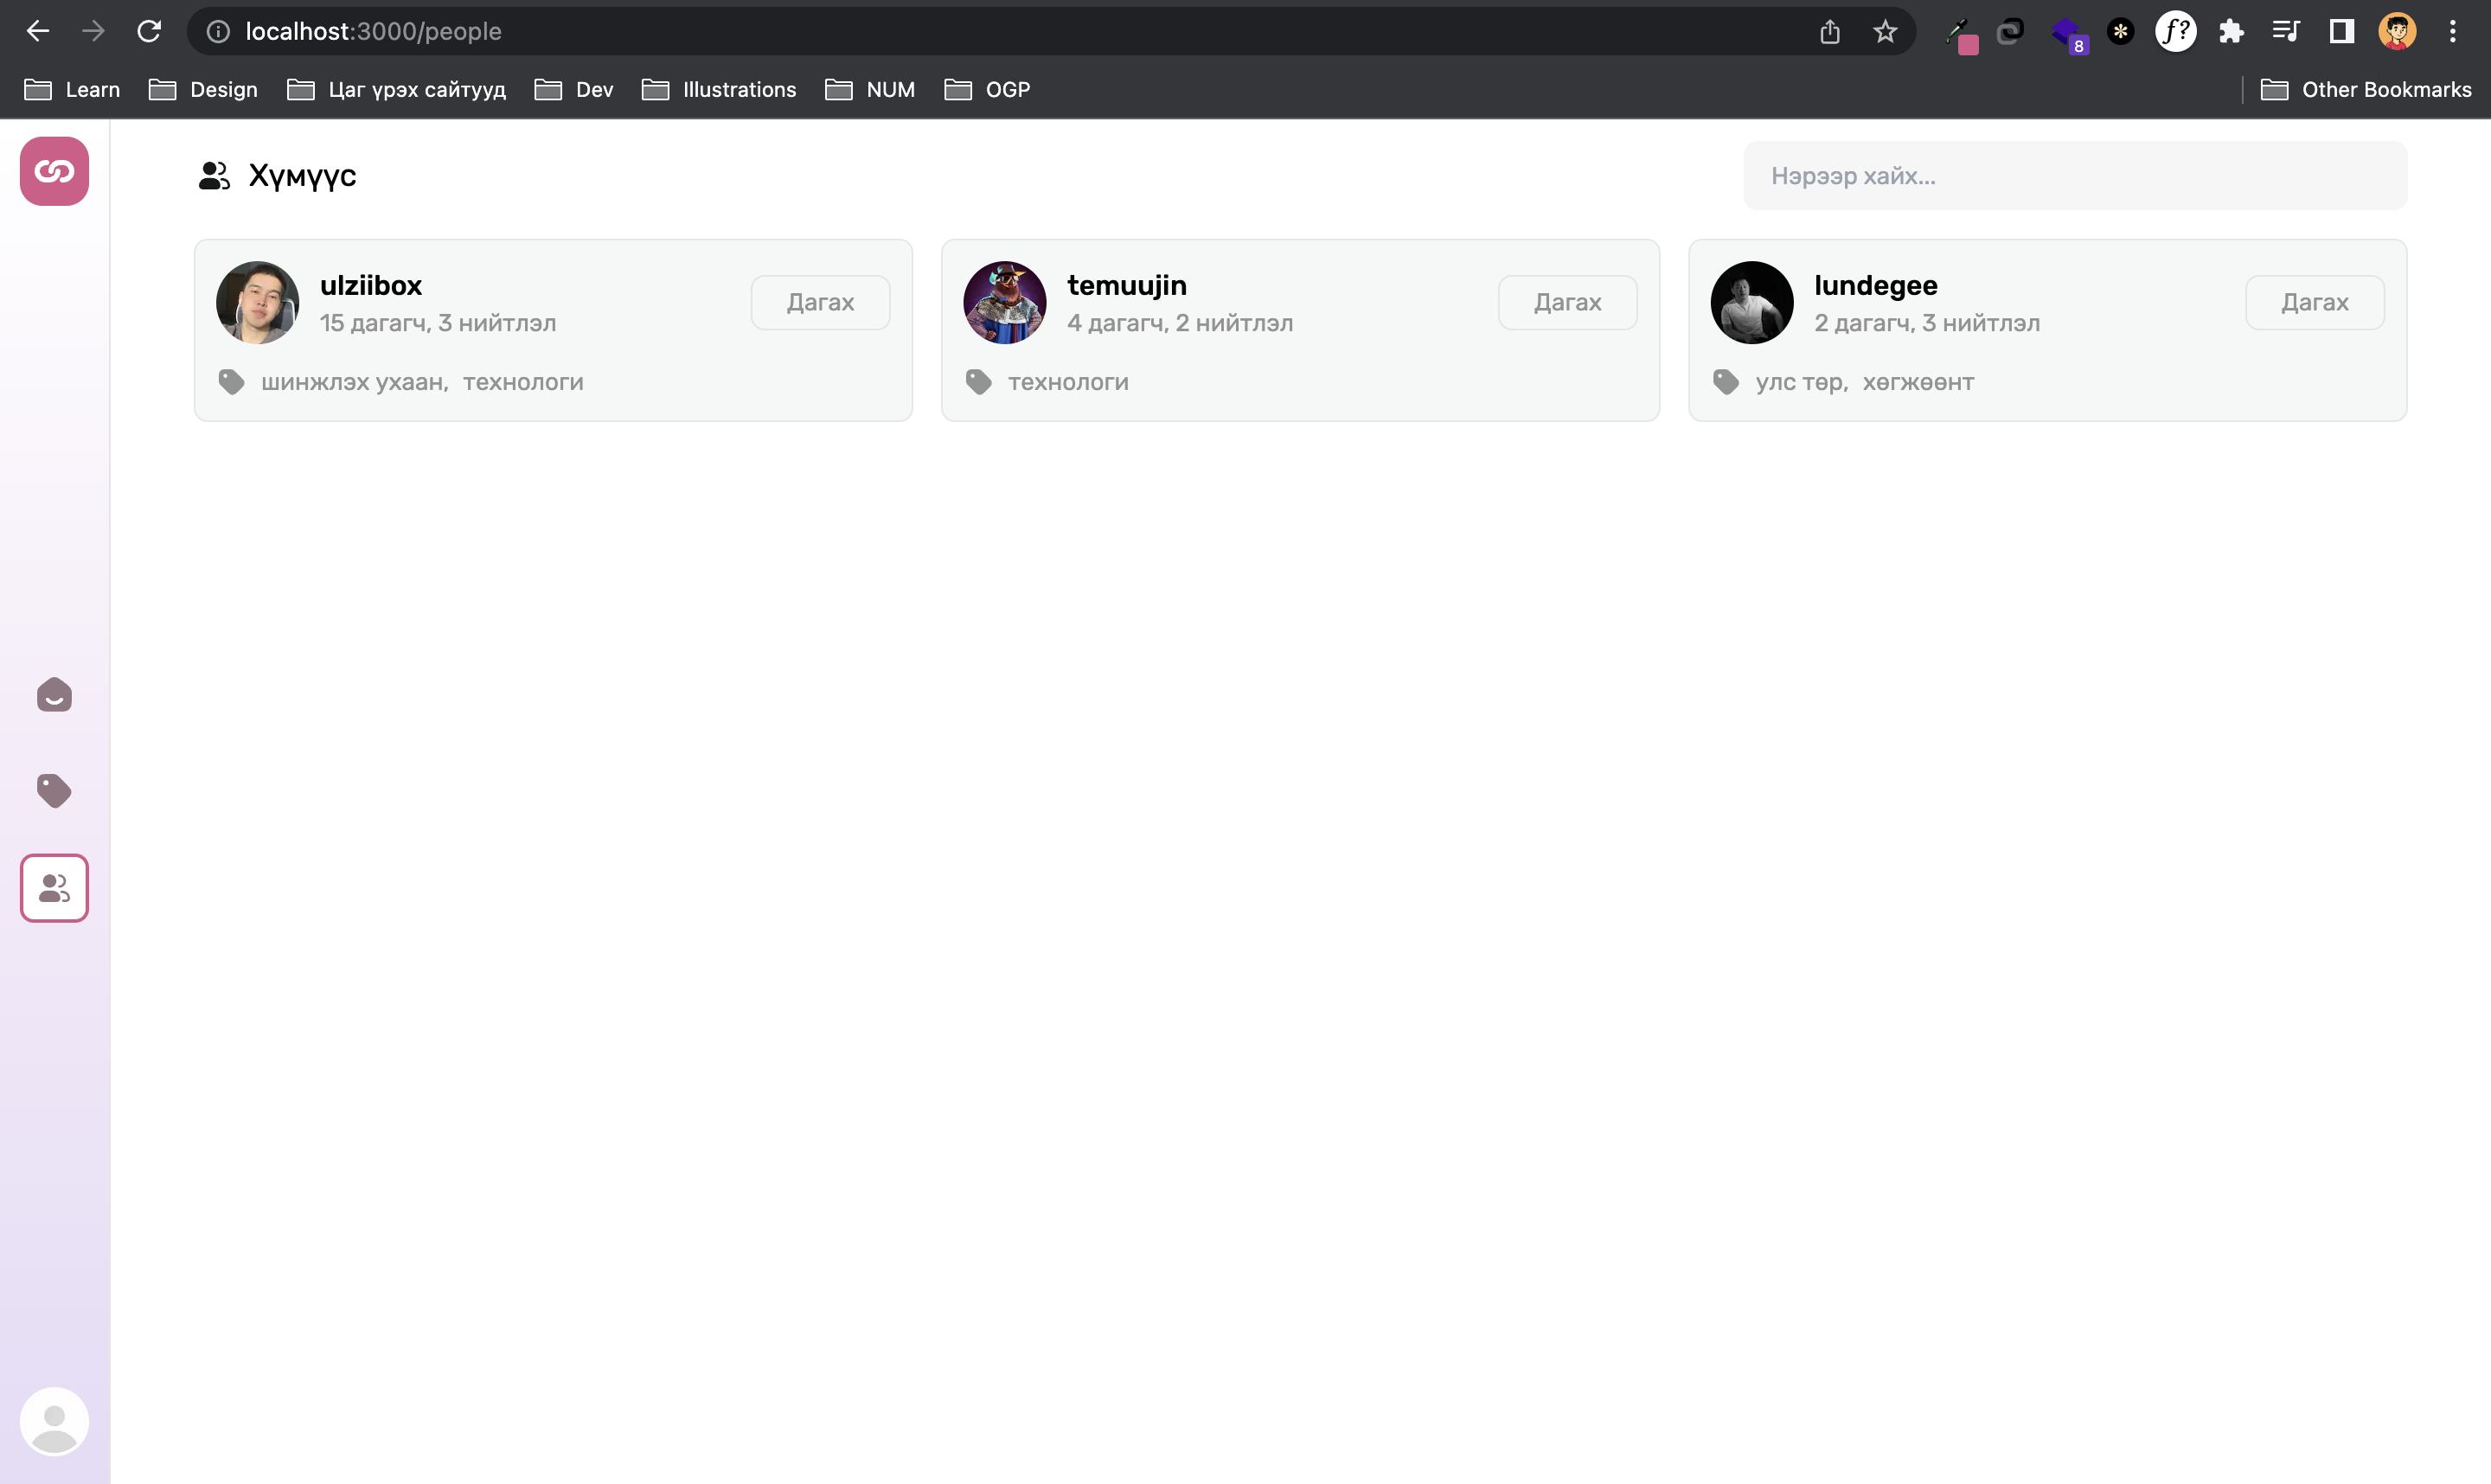
\includegraphics[width=13cm]{images/implement/users.png}
	\caption{Платформ дээр бүртгүүлсэн хэрэглэгчдийн жагсаалтыг харах}
	\label{fig:people-list}
\end{figure}
